% tree_encoding.tex -- standalone source for Fig. "fig:tree-encoding"
% Build:  pdflatex tree_encoding.tex   ->  tree_encoding.pdf
% Use:    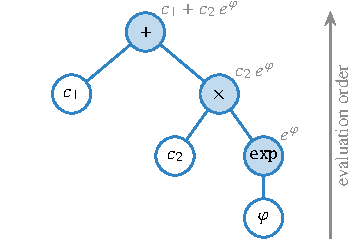
\includegraphics{tree_encoding.pdf}   (no width/scale option)
%
% Same class and font setup as the paper, so \small, \footnotesize and the
% math fonts are identical. preview crops the page to the TikZ bounding box,
% i.e. exactly the box the inline tikzpicture occupied.
\documentclass[10pt,prd,preprintnumbers,floatfix,aps,nofootinbib,twocolumn,superscriptaddress,noshowpacs]{revtex4-1}
\usepackage[utf8]{inputenc}
\usepackage{amssymb}
\usepackage{amsmath}
\usepackage{amsfonts}
\usepackage{amsbsy}
\usepackage[dvipsnames]{xcolor}
\usepackage[T1]{fontenc}
\usepackage{newtxtext}
\usepackage{newtxmath}
\usepackage[cal=cm]{mathalfa}

\usepackage{tikz}
\usetikzlibrary{positioning,arrows.meta,fit,backgrounds,shapes.geometric,calc}
\definecolor{treeblue}{RGB}{48,132,196}
\definecolor{treebluedark}{RGB}{35,100,150}

\usepackage[active,tightpage]{preview}
\PreviewEnvironment{tikzpicture}
\setlength\PreviewBorder{0pt}

\begin{document}
\begin{tikzpicture}[
    level distance=10.5mm,
    level 1/.style={sibling distance=25mm},
    level 2/.style={sibling distance=15mm},
    edge from parent/.style={
        draw=treeblue,
        line width=0.85pt
    },
    treenode/.style={
        circle,
        draw=treeblue,
        text=black,
        line width=0.85pt,
        minimum size=6.5mm,
        inner sep=0pt,
        font=\small
    },
    op/.style={treenode, fill=treeblue!30!white},
    leaf/.style={treenode, fill=white},
    sub/.style={font=\small, text=black!45, inner sep=0.5pt},
    evalarrow/.style={
        draw=black!45,
        line width=0.85pt,
        -{Stealth[length=2.2mm,width=1.8mm]}
    }
]

\node[op, label={[sub]above right:$c_1 + c_2\,e^{\varphi}$}] (root) {$+$}
    child {
        node[leaf] {$c_1$}
    }
    child {
        node[op, label={[sub]above right:$c_2\,e^{\varphi}$}] {$\times$}
        child {
            node[leaf] {$c_2$}
        }
        child {
            node[op, label={[sub]above right:$e^{\varphi}$}] {\texttt{exp}}
            child { node[leaf] (phi) {$\varphi$} }
        }
    };

% Remember the horizontal centre of the tree (nodes + gray labels) before
% anything else is added.
\coordinate (treeC) at (current bounding box.center);

% Evaluation-order arrow: placed 3 mm to the right of everything drawn so far
% (tree + gray labels), running from the leaf level up to the root level.
\coordinate (evalx) at ($(current bounding box.east)+(5mm,0)$);
\draw[evalarrow] (evalx |- phi.south) -- (evalx |- root.north)
    node[midway, sloped, below, font=\small, text=black!45, inner sep=2pt]
    {evaluation order};

% Invisible point mirroring the right edge about treeC, so the bounding box
% is symmetric and the tree stays centred when the PDF is centred in the column.
\path ($(current bounding box.east)!2!(treeC)$);

\end{tikzpicture}
\end{document}